\section{Task-Relevant Motion in Local Moment Space}
\label{sec:task-geometry}
\subsection{An exact bridge beyond independent frequencies}
For valid patches $p_u(x)\in\R^p$, define
\begin{equation}
 M(x)=|U|^{-1}\sum_u p_u(x)p_u(x)^\top.
\end{equation}
Squaring and GAP give $r_c(x)=h_c^\top M(x)h_c$ for every input. Let $\phi=\operatorname{svec}(M-\E M)$, where symmetric vectorization preserves the Frobenius inner product. Write its covariance on its support as $\Sigma_\phi=U\Lambda U^\top$, $\Lambda\succ0$, and set
\begin{align}
 u&=\Lambda^{-1/2}U^\top\phi,\qquad \E uu^\top=I,\\
 B_{c:}&=\operatorname{svec}(h_ch_c^\top)^\top U\Lambda^{1/2},\qquad A=WB.
\end{align}
Thus the centered encoder and projection are exactly $Bu$ and $Au$. Gaussianity and independent frequency powers are unnecessary for this identity. They remain useful for explicit dynamics and exact moment calculations.

For any centered multi-output label $Y$ with finite second moment, put $C_Y=\E[uY^\top]$ and $T=C_YC_Y^\top$. Population affine least squares gives
\begin{equation}
 R(A)=\tr\operatorname{Cov}(Y)-\tr(P_AT).
 \label{eq:general-task-risk}
\end{equation}
This standard regression identity includes coordinate, band-energy, and centered one-hot tasks without assuming that labels are linear functions of $u$. It describes linear readability, not all task information or finite-sample probe generalization. Below, moment-space training formulas assume augmented moments are supported on the same clean covariance support. If augmentation introduces clean-null directions, training must retain those additional coordinates; clean whitening alone does not determine its gradient.

\subsection{Data anisotropy and parameter mobility are separate sources}
Assume the representation matrix under discussion has full row rank on the interval. Write $P=P_A$, $Q=I-P$. For an effective update $Z$, its projector tangent is
\begin{equation}
 \mathcal D_A[Z]=A^\dagger ZQ+QZ^\top(A^\dagger)^\top.
 \label{eq:projector-tangent}
\end{equation}
Only $ZQ$ can change its row space. If $G=\nabla_A L$, ordinary parameter training induces
\begin{equation}
 \dot A=-\eta_h\mathcal M_h[G]-\eta_WGB^\top B,
 \label{eq:mobility-split}
\end{equation}
where $\mathcal M_h=J_hJ_h^*$ and $J_h=D_h(WB)$. Total gradient size and feature energy do not determine either projector tangent.

There is a concrete near-isotropy version of linear conservation. Decompose $G=HA+E$ and let $A=WV$ be a linear factorization. Then
\begin{equation}
 \dot V(I-P_V)=-\eta_VW^\top E(I-P_V).
 \label{eq:linear-leakage}
\end{equation}
For GUPA let $S=sI+\Delta S$, $D=d_0I+\Delta D$, and
\begin{equation}
 K=(I+ASA^\top)^{-1}+(I+ASA^\top)^{-2}.
\end{equation}
Its exact gradient is $G=AD-KAS$, so one may take
\begin{align}
 H&=d_0I-sK,\qquad E=A\Delta D-KA\Delta S,\\
 \norm E_F&\le\norm A_F(\norm{\Delta D}_2+2\norm{\Delta S}_2).
 \label{eq:gupa-residual}
\end{align}
The isotropic term cannot move the encoder row space; the residual can have a systematic finite-data component. Under exact isotropy this conservation also holds for ordinary discrete gradient descent whenever the front matrix retains its rank, since each update is a left multiplication.

For the square encoder, let $J_c=D_{h_c}B_{c:}^\top$, $T_c=J_cJ_c^\top=\tau_c I+\mathcal E_c$, and $U_0=W^\top HW$. With $Q_B=I-P_B$, its exact exterior velocity is
\begin{equation}
 (\dot BQ_B)_{c:}=-\eta_h\big[(U_0B)_{c:}\mathcal E_c
 +(W^\top E)_{c:}T_c\big]Q_B.
 \label{eq:square-leakage}
\end{equation}
This separates parameter-mobility anisotropy from objective/data anisotropy. A square parameterization does not automatically move its encoder space: scalar channel mobilities $T_c=\tau_cI$ and $E=0$ exclude that motion. Conversely, anisotropic channel mobilities can move it even when $E=0$. Appendix~\ref{app:task-geometry} gives a two-filter criterion: for isotropic Gaussian patches and linearly independent filters, motion occurs exactly when filter correlation and objective/head cross coupling are both nonzero.

\subsection{A solvable encoder rebound family}
\label{sec:bottleneck-family}
The following family makes the mechanism explicit in a genuine bottleneck $K=1<C=2<d=3$. Its moving directions are coupled quadratic statistics, not an embedding with dormant extra coordinates.

Let $x\sim N(0,\Sigma_x)$ be one two-dimensional patch, with
\begin{equation}
 \Sigma_x=\nu_+e_+e_+^\top+\nu_-e_-e_-^\top,
 \qquad \nu_\pm\in[19/20,21/20],
\end{equation}
where $e_+,e_-$ are orthonormal. Write $q_c=\Sigma_x^{1/2}h_c$ for the filters in whitened input coordinates, and initialize
\begin{align}
 q_1&=\sqrt\epsilon\,e_++\sqrt{\epsilon/2}\,e_-,\\
 q_2&=\sqrt\epsilon\,e_+-\sqrt{\epsilon/2}\,e_-,\qquad W=(w_0,w_0).
\end{align}
Set $E_\pm=e_\pm e_\pm^\top$ and $E_\times=(e_+e_-^\top+e_-e_+^\top)/\sqrt2$. These give orthonormal coordinates for
\begin{equation}
 u=\operatorname{svec}(yy^\top-I)/\sqrt2,\qquad y=\Sigma_x^{-1/2}x.
\end{equation}
For tasks use the unit vector associated with the symmetric matrix
\begin{equation}
 \beta_{\psi,z}=\sqrt{1-z^2}(\cos\psi E_++\sin\psi E_-)+zE_\times.
\end{equation}

\begin{theorem}[Uniform encoder and projection risk gaps]
\label{thm:bottleneck-family}
Let $0<\epsilon\le1/100$, $0<w_0\le1/10$, $\eta_h>0$, and $0\le r=\eta_W/\eta_h\le10$. Use GUPA with views $x+\xi_j$, where independent $\xi_j\sim N(0,\eta\Sigma_x)$ and $0\le\eta\le1/5$. Train the actual Euclidean parameters $h,W$. Put $\theta_0=\arctan(1/2)$. For every task $Y=\beta_{\psi,z}^\top u$ with
\begin{equation}
 2\theta_0/3\le\psi\le5\theta_0/6,\qquad |z|\le1/2,
\end{equation}
the same two comparison states $t_1<t_2$ satisfy, for both optimal encoder and projection risks,
\begin{align}
 R(t_1)&\le R(0)-\Delta_1,\\
 R(t_2)&\ge R(0)+\Delta_2,
\end{align}
where
\begin{align}
 \Delta_1&=\tfrac34\sin(\theta_0/4)\sin(\theta_0/12)>0.00335,\\
 \Delta_2&=\tfrac34\sin(5\theta_0/6)\sin(\theta_0/6)>0.02181.
\end{align}
Both states are reached before $t_2<5/(76\eta_hw_0^2\epsilon)$; the loss strictly decreases and the encoder/projection ranks remain two/one. Changing $r$ in this family changes speed and energy, but not the ordered subspace path or these gaps.
\end{theorem}

\paragraph{Mechanism and exact solution.}
Equal head entries and the displayed filter symmetry persist. Put $\lambda_\pm=\norm{q_1}^2\pm q_1^\top q_2$ and $\kappa=2\Phi'(V)$ for the radial objective $L=\Phi(V)$, $V=\norm A^2$. In the increasing clock $\tau=-8\eta_h\int\kappa w^2dt$,
\begin{align}
 \lambda_\pm(\tau)&=\frac{\lambda_\pm(0)}{1-\nu_\pm\lambda_\pm(0)\tau},\\
 w^2&=w_0^2+\frac r4\sum_{j\in\{+,-\}}
             \frac{\lambda_j-\lambda_j(0)}{\nu_j}.
 \label{eq:analytic-family}
\end{align}
The encoder retains $E_\times$ and the diagonal direction $\lambda_+E_++\lambda_-E_-$; the projection retains only the latter. Its angle $\theta=\arctan(\lambda_-/\lambda_+)$ strictly decreases. The task risks are exactly
\begin{align}
 R_{\rm enc}&=(1-z^2)\sin^2(\theta-\psi),\\
 R_{\rm proj}&=z^2+(1-z^2)\sin^2(\theta-\psi).
 \label{eq:analytic-risks}
\end{align}
The two common states are $\theta_1=3\theta_0/4$ and $\theta_2=\theta_0/6$. Motion first approaches the task direction and then continues past it; the encoder itself loses readability. The fixed projection gap $z^2$ is a separate selection effect.

\begin{figure}[t]
\centering
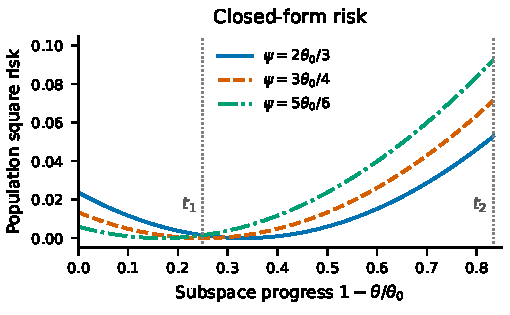
\includegraphics[width=\linewidth]{figures/analytic_bottleneck_family.pdf}
\caption{Exact risk paths in Theorem~\ref{thm:bottleneck-family}, three task directions with $z=0$. Encoder and projection risks coincide here. The same two comparison states improve and then exceed the initial risk for the entire task family. These curves evaluate the closed formula; no model is trained or numerically integrated to draw them.}
\label{fig:analytic-family}
\end{figure}

The task family contains an open cone and covers a specified $\pm5\%$ covariance range. This anisotropy range keeps covariance axes aligned with filter sums/differences and uses covariance-relative augmentation and balanced whitened initialization. Physical initial filters change with the covariance to keep that whitened balance. It is not robustness to arbitrary symmetry-breaking initialization or augmentation perturbations, nor a random-initialization probability result. The family also supplies an explicit exclusion case for rate competition: unequal rates alone do not force different directional paths. Appendix~\ref{app:task-geometry} proves the formulas, energy barrier, and reachability.


\subsection{How much motion can matter to a task?}
Let $P_0,P_1$ be equal-rank projectors, $Q_0=I-P_0$, and define
\begin{equation}
 a_0=\norm{Q_0TP_0}_F,\qquad d_{01}=\norm{P_1-P_0}_F/\sqrt2.
\end{equation}
The task cross block $a_0$ and the subspace displacement constrain risk jointly:
\begin{equation}
 |R(P_1)-R(P_0)|\le2a_0d_{01}
 +\operatorname{osc}(T)d_{01}^2,
 \label{eq:finite-motion-bound}
\end{equation}
where $\operatorname{osc}(T)=\lambda_{\max}(T)-\lambda_{\min}(T)$. This follows from the exact row/normal block decomposition in Appendix~\ref{app:task-geometry}, rather than a fitted local slope. In particular, $a_0=0$ excludes a first-order change, but can permit a one-sided quadratic change. If the row block of $T$ has eigenvalues at least $\delta>0$ above those of the normal block and $a_0=0$, every departure raises risk by at least $\delta d_{01}^2$.

For a parameter path with cumulative update budget
\begin{equation}
 b=\int(\norm{\dot h}_F+\norm{\dot W}_F)\,dt,
\end{equation}
suppose a containing region has $\sigma_{\min}(A)\ge\sigma>0$ and $\norm{DA[v]}_F\le J\norm v$. Then $d_{01}\le Jb/\sigma$, and Equation~\eqref{eq:finite-motion-bound} holds with this upper bound for every rate schedule in the region. A sharper bound uses $\int\norm{A^\dagger\dot A(I-P_A)}_Fdt$. For the linear encoder, Equation~\eqref{eq:linear-leakage} bounds that integral by
\begin{equation}
 \int\eta_V\norm{V^\dagger W^\top}_2
              \norm{E(I-P_V)}_F\,dt.
\end{equation}
This is a quantitative near-conservation statement. Constants inferred from future states give an a posteriori bound; source-fixed region bounds give a forward guarantee. None of these quantities is controlled by spectral concentration alone.

\subsection{Competition, duration, and an error budget}
Let $D_h,D_W$ be the two unit-rate projector tangents at a common state. A structural criterion is available before selecting a task: if either tangent vanishes, or if $D_W=\lambda D_h$ for some $\lambda>0$, no PSD task matrix admits opposing contributions. Otherwise an open family of rank-one tasks does admit competition. This is an if-and-only-if statement; its proof uses the off-diagonal block structure of projector tangents (Appendix~\ref{app:task-geometry}). It does not put a given class-label task in that family.

To specify an actual update budget, normalize the negative block gradients to unit directions $u_h,u_W$ and write
\begin{equation}
 \frac{d\theta}{db}=\alpha u_h+(1-\alpha)u_W.
\end{equation}
The sum of block path speeds is one. Fixed $\alpha$ generally requires a state-dependent physical rate ratio. On a source-centered ball of radius $\rho$, assume $\norm{\nabla R}\le G_R$, $\norm{\nabla^2R}\le H_R$, and $\operatorname{Lip}(u_g)\le K$. Put $L_q=H_R+G_RK$ and $q_g=\langle\nabla R_0,u_{g,0}\rangle$. For every allocation schedule and $b\le\rho$,
\begin{align}
 b\min_g q_g-\tfrac12L_qb^2
 &\le R(b)-R_0\nonumber\\
 &\le b\max_g q_g+\tfrac12L_qb^2.
 \label{eq:budget-envelope}
\end{align}
For fixed allocations with initial slopes at least $m$ and at most $-m$, both signs persist up to $b\le\min\{\rho,m/(2L_q)\}$; each change has magnitude at least $mb/2$. Any two schedules differ in risk by at most $b|q_h-q_W|+L_qb^2$.

With Euler steps of size at most $\delta_{\max}$ and normalized direction error at most $\varepsilon$, the usable margin becomes
\begin{equation}
 m_{\rm eff}=m-G_R\varepsilon
 -\tfrac12H_R(1+\varepsilon)^2\delta_{\max}.
 \label{eq:margin-budget}
\end{equation}
If it is nonpositive, this certificate supplies no sign guarantee. If it is positive, a sufficient cumulative window is
\begin{equation}
 b\le\min\left\{\frac\rho{1+\varepsilon},
 \frac{m_{\rm eff}}{L_q(1+\varepsilon)}\right\},
\end{equation}
with signed change at least $m_{\rm eff}b/2$. These are explicit sufficient bounds, not predictions that CIFAR errors are small. Appendix~\ref{app:task-geometry} supplies source-computable derivative constants and distinguishes this path budget from a fixed sum of learning rates. The generic Taylor bound is a connecting tool; its nonvacuity must be checked separately.

\subsection{Task-directed stochastic windows and abstention}
\label{sec:task-stochastic}
For stochastic training, a source tangent must compete with both mean error and centered fluctuation. Fix a source $\vartheta_0$, task $T$, rate ratio, and horizon $H$ before the independent mean/variance calibration. Write the actual finite-batch update as
\begin{equation}
 \vartheta_{j+1}=\vartheta_j+\delta_jF(\vartheta_j,\zeta_j).
 \label{eq:stoch-update}
\end{equation}
Here $\zeta_j$ contains an entire batch and its augmentations. In particular, the expectation of the sample-centered GUPA gradient need not equal its population gradient. We predict the specified batch algorithm, without replacing its random moments by population moments.

Let $P=P_j$, $Q=I-P$, $P'=P_{j+1}$, $K_j=QP'P$, and $s_j=\norm{P'-P}_F/\sqrt2$. At unchanged rank, exact projector geometry gives
\begin{align}
 D_j:=R_{j+1}-R_j&=-2\langle QTP,K_j\rangle_F+B_j^{(2)},\\
 |B_j^{(2)}|&\le\omega s_j^2,\qquad \omega=\operatorname{osc}(T).
 \label{eq:stoch-cross-leakage}
\end{align}
Thus $D_j=\E_jD_j+\xi_j$ has a scalar martingale error. Its conditional variance satisfies
\begin{equation}
 \sqrt{\operatorname{Var}_j(D_j)}
 \le2\sqrt{\operatorname{Var}_j\langle QTP,K_j\rangle_F}
       +\omega\sqrt{\E_js_j^4}.
 \label{eq:stoch-task-variance}
\end{equation}
Task-cross norm alone does not identify this variance: the orientation of random normal motion matters. If $QTP=0$, first-order noise vanishes but quadratic leakage remains. For example, when $T=\lambda P$, $D_j=\lambda s_j^2$ exactly; unbiased parameter noise can increase expected task risk. Appendix~\ref{app:task-stochastic} also gives two tasks with identical cross norms and geometric displacement but different exact finite-step variances.

Set $q(\vartheta,\zeta)=\langle\nabla R,F\rangle$ and $b_n=\sum_{j<n}\delta_j$. Independent source batches estimate its mean by $\widehat q_0$, with a confidence error $a$ and a variance upper confidence bound. This differs from using an observed absolute-error quantile as a uniform noise bound.
\begin{proposition}[Finite-prefix stochastic envelope]
\label{prop:stoch-prefix}
Assume fresh whole batches with the calibration law, a rank-preserving parameter ball of radius $\rho$, and uniform bounds
\begin{align}
 \norm F&\le M,&\operatorname{Lip}(F)&\le K_F,\nonumber\\
 \norm{\nabla R}&\le G_R,&\norm{D^2R}&\le H_R.
\end{align}
If $Mb_H\le\rho$, put $L_q=H_RM+G_RK_F$. With total failure probability at most $\varepsilon_{\rm cal}+\varepsilon_f$, all $1\le n\le H$ satisfy
\begin{align}
 |R_n-R_0-b_n\widehat q_0|\le{}&a b_n
 +\tfrac12L_qM\big(b_n^2-\sum_{j<n}\delta_j^2\big)\nonumber\\
 &+\tfrac12H_RM^2\sum_{j<n}\delta_j^2
 +\mathcal B_{\varepsilon_f}(\overline V_n).
 \label{eq:stoch-four-errors}
\end{align}
Here $\overline V_n$ bounds the accumulated conditional variance of the centered task slopes $\delta_jq_j$; $\mathcal B$ is the simultaneous scalar boundary specified in the appendix.
\end{proposition}
The four terms are source calibration, state drift, step curvature, and centered random fluctuation. The nominal clock $b_n$ is not parameter path length; $Mb_H\le\rho$ supplies that conversion. The appendix provides computable source variance confidence bounds and an exact finite-step alternative that retains quadratic noise inside the variance.

Issue a direction only when the resulting interval excludes zero, or a specified practical risk threshold. A useful prefix may follow a burn-in period; that certifies the selected later prefixes, not a sign at every earlier prefix. Simultaneous interval coverage holds from prefix one, including abstaining prefixes. A claim of one sign throughout $1{:}H$ requires every corresponding interval to exclude zero.

The existing texture predictor already projects its calibration errors into each task direction. Its empirical radius accumulates $H$ times an absolute task-error quantile. The proposed refinement separates source mean error from centered variance and accumulates the latter through $\overline V_n$; probability concentration itself is classical~\cite{freedman1975tail,howard2020timeuniform}. Current saved quantiles do not instantiate the required upper confidence and support bounds. The eight-stream decomposition contains substantial mean-offset and dispersion contributions, and no nonempty strict stochastic window is established here.


\subsection{A nonempty forward window on existing trajectories}
\label{sec:origin-windows}
We test nonvacuity on three stored matched-function trajectories of the original two-frequency model. All start with $A_0=(0.02432,0.02432)$; the $c=1$ source is exactly the center of Theorem~\ref{thm:gap}. Source-only interval arithmetic bounds the physical vector field, risk acceleration, and first hitting time of $\ell=0.02$. It then opens the saved trajectory CSV for validation, without integrating a new trajectory. Table~\ref{tab:origin-windows} gives conservative outward display bounds.

\begin{table}[t]
\centering\small
\caption{Finite changes at the first common energy section $\ell=0.02$. Predictions use the source state only. Future entries are pre-existing numerical trajectories, not independent trials.}
\label{tab:origin-windows}
\setlength{\tabcolsep}{4pt}
\begin{tabular}{rcr}
\toprule
Scale $c$&Certified $R(\ell)-R(0)$&Saved change\\\midrule
$1/2$&$[0.003179,0.007176]$&$0.005326$\\
$1$&$[-0.003110,-0.001259]$&$-0.002280$\\
$3/2$&$[-0.010741,-0.002101]$&$-0.006647$\\
\bottomrule
\end{tabular}
\end{table}

The source bounds certify nonzero changes with opposite signs at the same initial function and common progress section; the first two have risk separation greater than $0.00443$. All saved hitting times and risks fall within their predicted intervals. The physical windows also contain five saved future records, all inside the amplitude envelopes. This is a retrospective check of a forward certificate, not a newly preregistered experiment. It supplies a finite-window counterpart to the local threshold on this construction family, not an independent validation of every general moment-space bound or a natural-image prediction. Appendix~\ref{app:origin-windows} gives the boxes, failed shorter energy-clock bounds, and the separate fixed-rate-sum comparison.
